\documentclass[pre,twocolumn,preprintnumbers,reprint]{revtex4}
\usepackage{amsmath,amssymb}

\usepackage{overpic,color}
\newcommand{\ud}{\,\emph{d}}
\newcommand{\dd}{\mathrm{d}}
\newcommand{\pp}{\partial}
\newcommand{\intn}{\!\!\int\!}
\newcommand{\bu}{{\bf u}}
\newcommand{\br}{{\bf r}}
\newcommand{\rd}{{\rm d}}
\newcommand{\be}{\begin{equation}}
\newcommand{\en}{\end{equation}}


\usepackage{amssymb}
\usepackage{amsmath}
\usepackage[T1]{fontenc}
\usepackage{amsfonts}
\usepackage{graphicx}% Include figure files
\usepackage{subfigure}
\usepackage{dcolumn}% Align table columns on decimal point
\usepackage{bm}% bold math
\usepackage{hyperref}
\usepackage{empheq}
\usepackage{natbib}
\usepackage{color}
\newcommand*{\citen}{}% generate error, if `\citen` is already in use
\DeclareRobustCommand*{\citen}[1]{%
  \begingroup
    \romannumeral-`\x % remove space at the beginning of \setcitestyle
    \setcitestyle{numbers}%
    \cite{#1}%
  \endgroup
}

\begin{document}
\preprint{Version 0.8}

\title{Supplementary information: geometrically frustrated, two-dimensional nematics confined by a rectangular box
}

\author{Xiaomei Yao and Hui Zhang\footnote{Email: hzhang@bnu.edu.cn }}
\affiliation {School of Mathematical Sciences, Beijing Normal
University, Beijing 100875, P.R. China  }
\date{\today}

\author{Jeff Z. Y. Chen\footnote{Email: jeffchen@uwaterloo.ca}}
\affiliation{ Department of Physics and Astronomy, University of Waterloo, Waterloo, Ontario, Canada, N2L 3G1 }
\date{\today}


\maketitle


\section*{Visualization of the nematic structures}

The calculated physical properties are based on the distribution function of segments on a rodlike molecule, $f(\br, \bu)$. It is related to the center-of-mass distribution function  $\rho \left (\br , \bu \right )$ by
\begin{equation}\label{fdef}
f(\br,\bu) = {ab\over n} \int_0^1 \rho \left [\br - \bu L(s-{1\over 2}), \bu \right ] \dd s,
\end{equation}
where we trace back along the path of a rodlike molecule from the center of mass. The integrant
represents the probability density of finding the segment labeled by $s$ on the rodlike molecule, to appear on a location with the coordinate $\br$. The path-averaged $f(\br,\bu)$ is the probability density of finding {\emph{any segments}}, regardless of its label $s$, to appear at $\br$.
%Under the definition of the reduced mean density
%\begin{equation}\label{rhodef}
%\tilde \rho_0 \equiv L^2 n/ab,
%\end{equation}
With this definition $f(\br,\bu)$ is dimensionless and normalized to the box area $ab$.
In 2D, $f(\br, \bu)$ is expressed by $f(x,y; \theta)$ where $x,y$ are the Cartesian coordinates along the two perpendicular sides of a rectangle and $\theta$ is the angle between $\bu$ and the $x$-axis. Here a number of physical quantities are introduced to illustrate the nature of the three-variable function $f(x,y; \theta)$.

The density variation is reflected by the function
\begin{equation}\label{1}
\phi(x,y)=\int_0^{2\pi}f(x,y,\theta) \rd\theta
\end{equation}
where the $\theta$ dependence of the distribution function is averaged out. In the bulk isotropic and nematic states, this function is identically constant ($=1$). In the current system, the nematic defect locations normally accompany a low $\phi(x,y)$.

On a 2D surface, to measure the orientational ordering, we define the orientational order parameter tensor
\begin{equation}  \label{Qdef}
  \begin{split}
    {\sf Q}(x,y) &= {1\over 2} \left[\begin{array}{cc}
      S(x,y) & T(x,y)\\
      T(x,y) & -S(x,y)
    \end{array}\right],\\
  \end{split}
\end{equation}
where the two elements are
\be
S(x,y)=\frac{\int_0^{2\pi}\rd\theta\cos(2\theta)f(x,y,\theta)}{\phi(x,y)},
\en
\be
T(x,y)=\frac{\int_0^{2\pi}\rd\theta\sin(2\theta)f(x,y,\theta)}{\phi(x,y)}.
\en
Respectively, $S$ and $T$ characterize the ordering of the rodlike molecules along the $x$-axis and the direction that makes a $\pi/4$ angle with respect to the $x$-axis. Note that both $S$ and $T$ defined here have been divided by $\phi(x,y)$ whereas similar quantities studied in Ref. \citen{Chen2013} were directly the integrals in the numerators.

Based on this definition, the main order parameter measured from a local nematic director ${\bf n}(x,y)$ is found from the positive eigenvalue of the $\sf Q$-tensor,
\begin{equation}\label{lambda}
\Lambda (x,y) = \sqrt{S^2(x,y)+T^2(x,y)}.
\end{equation}
The nematic-director field itself is projected on the Cartesian axes by
\begin{equation}\label{ndef}
{\bf n}(x,y) = {\hat x}\cos\theta_0(x,y) + {\hat y}\sin\theta_0(x,y)
\end{equation}
where $\theta_0$ is determined from
\begin{equation}\label{thetadef}
\cos\theta_0 (x,y) = {1\over 2}\left[1 + {S(x,y)\over\Lambda(x,y)}\right]
\end{equation}
The location where $\Lambda =0$ is considered as a defect point and hence $\bf n$ can not be defined.

In a typical optical experiment, to image the possible defect pattern, a liquid-crystal cell is placed between two crossed polarizers. To model the defect pattern seen by the experiments, here we assume that the first polarizer makes an angle $\alpha$ with respect to the $x$-axis.
After the light passes the liquid-crystal cell, the electric field $E$ makes a projection
  $E\cos(\alpha-\theta)$ after been screened by those molecular segments oriented in the $\theta$ direction. Another projection of $\sin(\alpha-\theta)$ along the axis of the second polarizer makes the final outcome of the light intensity proportional to
\begin{equation}\label{Idef}
I_\alpha(x,y) = {1\over 4}\int_0^{2\pi} \dd \theta [\sin(2\theta-2\alpha)]^2 f(x,y;\theta).
\end{equation}
Two typical scenarios are that the polarizers are directed along $x$- and $y$-axes [$\alpha=\pi/2)$] and along directions that make $\alpha=\pi/4$ angles with the $x$- and $y$-axes.


%\begin{figure}[!t]\centering
%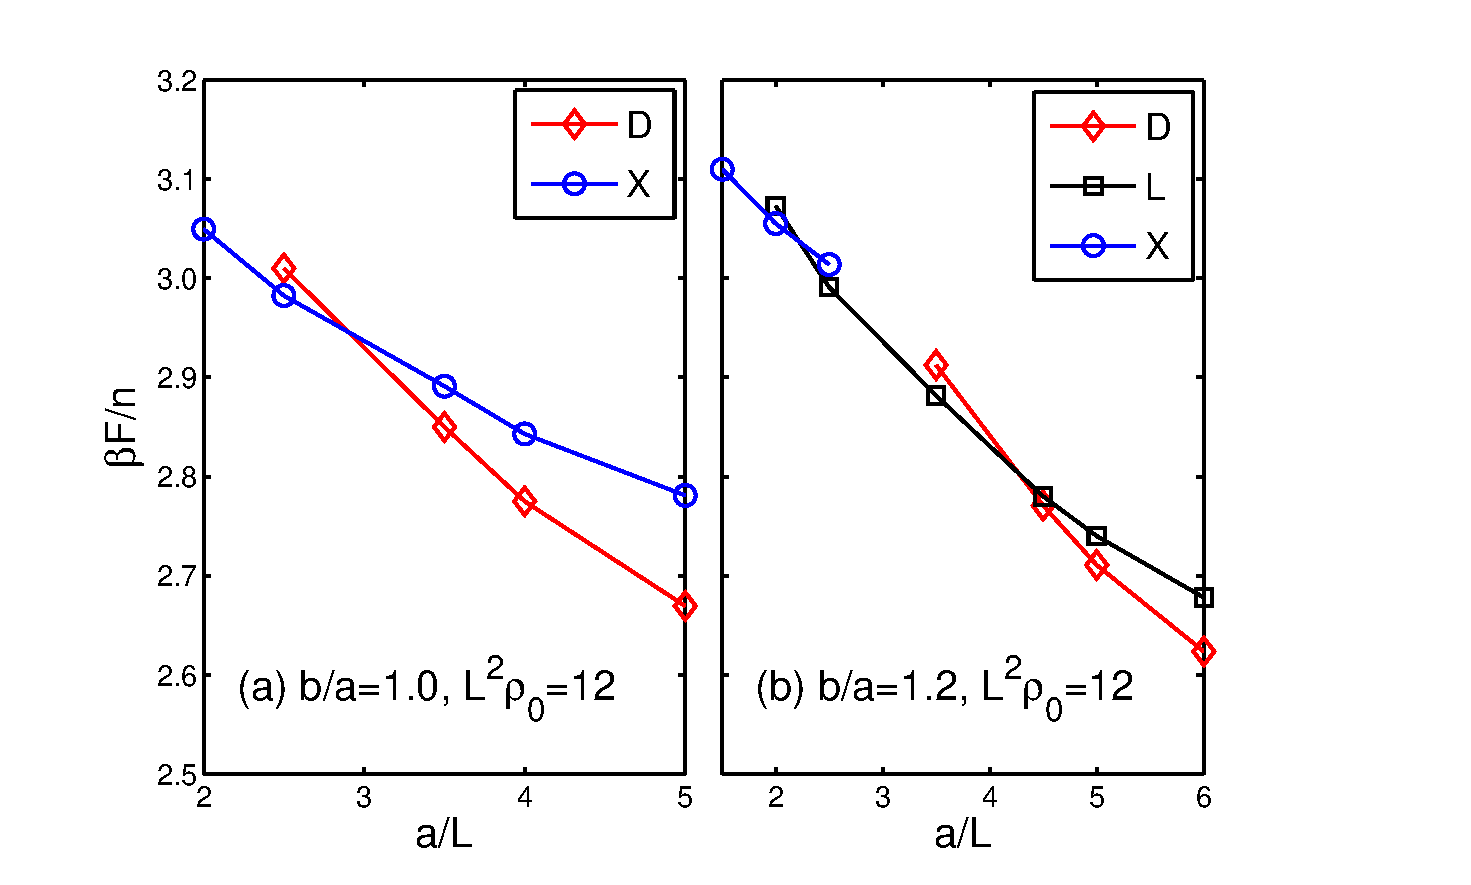
\includegraphics[width = 1.2 \columnwidth]{eps/energy-plot.eps}
%\caption{Two examples of the free-energy minima data as functions of $a/L$ for fixed (A) $[b/a, L^\rho_0]= [1,12]$ and (B)$ [1.2, 12]$. The crossing of these branches yields a phase boundary for the transition between the two involved states, of the first-order characteristics. } \label{P2}
%\end{figure}

%\begin{figure}[!t]
%\includegraphics[width = 0.85 \columnwidth]{eps/ABCD.eps}
%\caption{Phase diagrams for four given aspect ratios, plots (A)-(D) for $b/a=1, 1.2, 2, 3$, in terms of $a/L$ and $L^2\rho_0$. Refer to Figs. \ref{P1} and \ref{P4} for the defect structures that correspond to the labels of the stability regimes. A second-order phase transition curve (dashed) saparates the parameter space into ordered and isotropic (ISO) states.} \label{phase}
%\end{figure}


\section*{Self-consistent field theory}

The extended Onsager model presented in the text,
\begin{equation}
\begin{aligned}
\label{Fdef}
 \beta &F=\intn\rho(\mathbf{r},\mathbf{u}) \ln [L^2\rho(\mathbf{r},\mathbf{u}) ] {\rm d}\mathbf{r} {\rm d}\mathbf{u}\\
%&+\int \varrho(\mathbf{r},\mathbf{u}) \beta V(  \mathbf{r},\mathbf{u}  )  \;\dd\mathbf{r} \dd\mathbf{u}\\
&+ \frac{1}{2}\int\rho(\mathbf{r},\mathbf{u}) w(\mathbf{r},\mathbf{u};\mathbf{r}^\prime, \mathbf{u}^\prime)\rho(\mathbf{r}^\prime, \mathbf{u}^\prime) \;\dd\mathbf{r} ,%\dd\mathbf{u} \dd\mathbf{r}^\prime \dd\mathbf{u}^\prime,
\end{aligned}
\end{equation}
can be casted as a self-consistent field theory (SCFT) for wormlike polymers with an infinite persistence length (hence the molecules are rigid), summarized here. The proof for mathematical equivalence is carefully addressed in both Refs. \citen{Chen2013} and **COMMENT** \citen{Chen2016}. The formalism requires the introduction of a path variable $s$, continuously varying from one end of the molecule where $s=0$ to another end where $s=1$. The direction of the unit vector $\bu$ is assumed to point from $s=0$ to $1$. A segment on the rodlike molecule then carries a label $s$.

A few advantages can be gained by using the path-averaged distribution function within the SCFT. The second {\emph{nonlocal}} term in \eqref{Fdef} can now be simply written
with a local interaction kernal function without the complex structure of $w$; the {\emph {nonlocal}} boundary conditions at the walls can be handled through the {\emph {local}} boundary conditions of the reduced Green's function. The price that must be paid for these simpler expressions is the the more complicated entropy term. Instead of the {\emph {local}} expression shown in the first term of \eqref{Fdef}, in terms of $f(\br, \bu)$ a {\emph{nonlocal}} relationship now needs to be considered, which, within SCFT, is determined by the solution a partial differential equation.

The density function is related to the reduced Green's function $q(\br,\bu;s)$ by
\be \label{q4}
f(\br,\bu)= \frac{n}{\rho_0 Q}\int_0^1\dd s q(\br,\bu;s)q(\br,-\bu;1-s)
\en
where $Q$ is the single-chain partition function,
\be \label{q2}
Q=\int\rd\br\rd\bu q(\br,\bu;1).
\en
The reduced Green's function $q(\br,\bu;s)$ is introduced to describe the probability of finding a polymer segment of length $s$ with its terminal end locating at $\br$ and pointing at unit vector $\bu$. Given an external potential $W(\br,\bu)$, $q(\br,\bu;s)$ can be calculated by solving the modified diffusion equation (MDE)\cite{Chen2013}
\be \label{q1}
\frac{\partial}{\partial s}q(\br,\bu;s)=[-L\bu\cdot\nabla_\br-W(\br,\bu)]q(\br,\bu;s),
\en
where an initial condition $q(\br,\bu;s)=1$ is imposed.
In this work we already assumed that the persistence length of the polymer $\lambda \gg 1$ to model a rodlike polymer.

The free energy in extended Onsager model can be rewritten as {XIAOMEI: CHECK... NOT CORRECT...}**COMMENTS**
\begin{align}\label{q5}
\beta F=&n\ln(\rho_0/Q)-\int\rd\br\rd\bu W(\br,\bu)\rho(\br,\bu)\nonumber\\
 &+\frac{1}{2}\rd\br\rd\bu\rd\bu'\rho(\br,\bu)|\bu\times\bu'|\rho(\br,\bu').
\end{align}
The minimization of \eqref{q5} with respect to $\rho(\br,\bu)$, $\delta (\beta F)/\delta\rho=0$ gives
\be \label{q6}
W(\br,\bu)=\rho_0\int\rd\bu'|\bu\times\bu'|f(\br,\bu'),
\en
which relates the mean-field $W$ with the distribution function.

The main logic of the self-consistent loop is the following. (A) The excluded-volume interaction of the system is modeled by the {\emph{local}} expression, \eqref{q6}. (B) For a single-chain statistics, $W$ is considered an external field and the reduced Green's function problem is solved through \eqref{q1} which yields the single-chain partition function through \eqref{q2} and probability distribution through \eqref{q4}. (C) One then goes back to \eqref{q6} to complete the self consistency.

The Onsager model ignores all fluctuation effects and hence is at a mean-field level. As such when it is used to model the isotropic-nematic phase transition of rodlike molecules in two-dimensions (2D), it predicts a second-order transition density \cite{Kayser1978,Cuesta1989,Chen1993},
\begin{equation}\label{ncriticql}
L^2 n^*/ab  = 3\pi/2,
\end{equation}
above which the nematic state is stable and below which the isotropic state is stable, where $ab$ is the area that contains the $n$ molecules. In the asymptotic limit $a/L \gg 1$ and $b/L \gg 1$, the confined system modeled here reduces back to this transition as the boundary effects diminish.

\section*{Boundary conditions}

Two main factors need to be implemented beyond the original Onsager model in two dimensions. One is the non-local $w(\mathbf{r},\mathbf{u};\mathbf{r}^\prime, \mathbf{u}^\prime)$ to treat the particle-particle interactions and the other, which also is non-local when using the center-of-mass coordinates, is the hard-wall potential acting on the molecules \cite{Holyst88,Chen1995,Koch1999,Roij01}.
%One of us has recently described the application of this model to the description of the nematic defect patterns present in square and circular boxes.

The wall-excluding potential can be easily handled by the use of the $q$ function \cite{Chen1995,Chen2013}, We let {XIAOMEI: CHECK... }**IT IS RIGHT**
\begin{equation}\label{q8}
    q(\br,\bu;s)=0 \quad ({\rm if}\,\bu \cdot  {\bf n}\ge 0\,\,{\rm and}\,s\neq0),
\end{equation}
where $\bf n$ is the normal direction of a wall area element, pointing to the box interior. The other half of function at the wall, for the parameter region $\bu \cdot  {\bf n}<0$ is specified automatically by the physical problem. The physical significance of this boundary condition, together with the consideration of the mathematical requirements in solving a partial differential equation within a hard-wall, is discussed much details in Sect. 2.5**COMMENTS** of Ref. \citen{Chen2016}. {XIAOMEI: complete}

\section*{Numerical algorithm to solve MDE}

The center of the numerical calculation is to solve MDE in \eqref{q1}. In this work we specify $\br$ through 2D variables $x,y$ and $\bu$ through the angle $\theta$ that it makes with the $x$ axis. Then the MDE can be represented by
\[
\frac{\partial}{\partial s}q(x,y,\theta;s)=[-L\cos\theta\frac{\partial}{\partial x}-L\sin\theta\frac{\partial}{\partial y}\]
\be\label{q7}
-W(x,y,\theta)]q(x,,y,\theta;s),
\en
with the initial condition
\be
q(x,y,\theta;0)=1.
\en
%As $q(x,y,\theta;s)$ is a four-variable function, it's a challenge to ensure its convergence and stability of the whole procedure
For numerical implementation, we assume that the parameter spaces in $x/L, y/L, \theta$ and $s$ are divided into $N_x, N_y, N_\theta$ and $N_s$ representative points; the nodes are labeled by integers $i,j,k$ and $n$. The function $q(x_i,y_j,\theta_k;s_n)$ is then directly represented by $q^n_{i,j,k}$. In most calculations, when $b/a=1$, we set $(N_x,N_y,N_\theta,N_s)$ to $(50,50,30,2000)$. In the large $b/a$ case, $N_y/N_x$ is adjusted accordingly. For example, when $b/a=2$, $(N_x,N_y,N_\theta,N_s)$ is set to $(50,100,30,2000)$.

In terms of $x$ and $y$, the above is a {\emph {first-order}} convection equation, which can be tackled by using the implicit upwind scheme. We write
%The implicit scheme is applied to make the whole procedure more efficient and stable, which is
\be
q_{i,j,k}^{n+1}=q_{i,j,k}^n+H_x q_{i,j,k}^{n+1}+H_yq_{i,j,k}^{n+1}+H_Wq_{i,j,k}^{n+1}.
\en
Here $H_W=-\Delta s W_{i,j,k}$ and the operators $H_x$ and $H_y$ yield
\be
H_xq_{i,j,k}^{n+1}=
\begin{cases}
-L \cos\theta_k\frac{\Delta s}{\Delta x}(q_{i,j,k}^{n+1}-q_{i-1,j,k}^{n+1}),\quad \cos\theta_k\geq0\\[3mm]
-L \cos\theta_k\frac{\Delta s}{\Delta x}(q_{i+1,j,k}^{n+1}-q_{i,j,k}^{n+1}),\quad \cos\theta_k<0
\end{cases},
\en
\be
H_yq_{i,j,k}^{n+1}=
\begin{cases}
-L \sin\theta_k\frac{\Delta s}{\Delta y}(q_{i,j,k}^{n+1}-q_{i,j-1,k}^{n+1}),\quad \sin\theta_k\geq0\\[3mm]
-L \sin\theta_k\frac{\Delta s}{\Delta y}(q_{i,j+1,k}^{n+1}-q_{i,j,k}^{n+1}),\quad \sin\theta_k<0
\end{cases}.
\en
Since the $\partial/\partial s$ operator is treated by Euler's forward scheme, the increment $\Delta s$ must be small enough to ensure numerical stability, which satisfies Courant-Friedrichs-Lewy condition\cite{Mahgerefteh2009}. **COMMENTS** [***PLEASE ADD REF***]

The above equations can be formally represented by the following notation,
\be
A(i,j,k)Q^{n+1}=Q^n.
\en
where we have moved all linear terms associated with the time step $n+1$ to the left-hand side. The $N_x\times N_y\times N_\theta$-dimensional matrix $A(i,j,k)$ contains all coefficients of these terms and is sparse, which can be inverted by using a standard algorithm. The $N_x\times N_y\times N_\theta$-dimensional vector $Q^{n+1}$ representing ${q_{i,j,k}^{n+1}}$ is then calculated at time step $n+1$ when $Q^{n}$ is given.

\begin{figure}[!t]
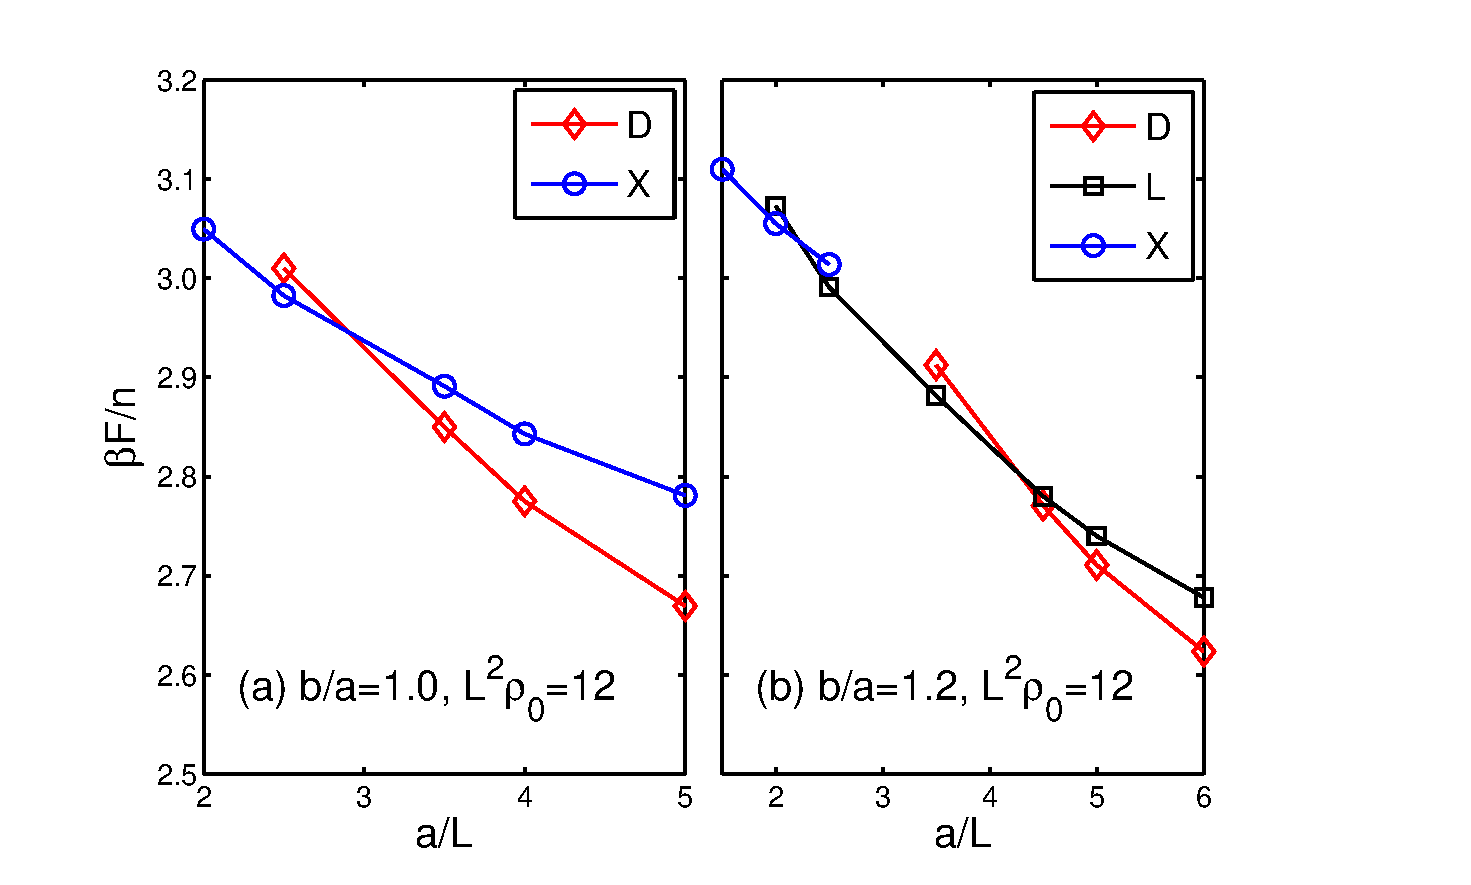
\includegraphics[width = 1.1 \columnwidth]{eps/energy-plot.eps}
\caption{Two examples of the free-energy minima data as functions of $a/L$ for fixed (a) $[b/a, L^2\rho_0]= [1,12]$ and (b)$ [1.2, 12]$.**COMMENT** The crossing of these branches yields a phase boundary for the transition between the two involved states, of the first-order characteristics. } \label{P2}
\end{figure}

\begin{figure}[!t]
\includegraphics[width = 0.85 \columnwidth]{eps/ABCD.eps}
\caption{Phase diagrams for four given aspect ratios, plots (a)-(d)**COMMENT** for $b/a=1, 1.2, 2, 3$, in terms of $a/L$ and $L^2\rho_0$. Refer to Figs. 1 and 2 in the text for the defect structures that correspond to the labels of the stable regions. A second-order phase transition curve (dashed) saparates the parameter space into ordered and isotropic (ISO) states.} \label{phase}
\end{figure}


\section*{Free energy and phase diagrams}


The relative stability of a defect state over the other can be assessed by examining the free-energy differences between these states. For example, each data point in Fig. \ref{P2}(a) **COMMENT** represents the free energy per particle, calculated after minimization is performed with respect to the probability density distribution, for a fixed $b/a=1$ and $L^2\rho_0 =12$. Interpolation of the calculated data indicates that a first-order phase transition takes place at $a/L \approx 2.9$ where, beyond this point, DS has a lower free-energy. This leads to the phase boundary in the phase diagram, Fig. \ref{phase}(a), at $[a/L, L^2 \rho_0]= [2.9,12]$. Calculations for other values of $L^2\rho_0$ give rise to the entire phase boundary curve for the SS-DS transition.

In another example, for a system with fixed $b/a=1.2$ and $L^2\rho_0=12$, by changing $a/L$ we obtain three free-energy branches corresponding to SS, VS, and DS, which are displayed in Fig. \ref{P2}(b). The first crossing point at $L^2 \rho_0 \approx 2.2 $ determines the SS-VS phase boundary and the second at $L^2 \rho_0 \approx 4.2$
the VS-SS phase boundary. Within this two points, both DS and SS are metastable.

Our system has three parameters, $[L^2 \rho_0, b/a, a/L]$. A complete phase diagram is hence dependent on three system parameters. Fig. \ref{phase} **COMMENT** is a series of two-dimensional phase diagrams with fixed values of the aspect ratio $b/a$. In the text, Fig.~4 is a phase diagram in terms of $[a/b, a/L]$, when $L^2\rho_0$ is fixed at $10$ **COMMENT**, above the isotropic-nematic transition curve.


\bibliography{Ref2,jy,LCC,yao,RefYSW} %You need to replace "rsc" on this line with the name of your .bib file

%\begin{thebibliography}{99}
%\end{thebibliography}
\bibliographystyle{apsrev4-1}
%\bibliographystyle{unsrt}
%theme:
%	plain: sort alphabetically based on author, year and title.
%	abbrv: abbreviation of plain style
% 	unsrt: sort based on the order of citation

%\onecolumngrid

%\vfill
%\newpage


\end{document}








































